\documentclass{article}%
\usepackage[T1]{fontenc}%
\usepackage[utf8]{inputenc}%
\usepackage{lmodern}%
\usepackage{textcomp}%
\usepackage{lastpage}%
\usepackage{geometry}%
\geometry{margin=0.7in}%
\usepackage{hyperref}%
\usepackage{graphicx}%
\usepackage{fancyhdr}%
%
\fancypagestyle{header}{%
\renewcommand{\headrulewidth}{0pt}%
\renewcommand{\footrulewidth}{0pt}%
\fancyhead{%
}%
\fancyfoot{%
}%
\fancyhead[L]{%
\vspace{0.5cm}%
\Large Group : CEN1.2B%
\linebreak%
\Large 1\textsuperscript{st} Year%
}%
\fancyhead[R]{%
\vspace{0.5cm}%
\Large Name : Necsulea Andrei-Mihai%
}%
\fancyfoot[C]{%
\thepage%
}%
}%
%
\begin{document}%
\normalsize%
\pagestyle{header}%

        \vspace*{\fill}
        \begin{center}
            \LARGE \textbf{ALGORITHM DESIGN HOMEWORK} \\
            \Large \textbf{- TECHNICAL REPORT -}
        \end{center}
        \vspace*{\fill}
    %
\newpage%
    
        \vspace*{\fill}     
        \begin{center}
            \LARGE \section{Homework assignment problem - The LOBSTERS Problem}
            \vspace{0.5cm}
        \end{center}
        \begin{Large}
        A fisherman is exploring a coastal region rich in lobsters, each with
        its own size (in centimeters) and value (in gold coins). The fisher-
        man’s net has a limited capacity, expressed in the total number of
        centimeters it can hold. Given a detailed list of the sizes and values
        of the lobsters available in that region, your task is to develop a strat-
        egy for the fisherman to select lobsters in such a way as to maximize
        the total value of his catch while adhering to the net’s capacity limit.
        You need to decide which lobsters to include in the net and which
        to leave behind so that the sum of the values of the selected lobsters
        is as high as possible, without the sum of their sizes exceeding the
        capacity of the net.
        
        \vspace{0.3cm}
        Imagine a scenario where a fisherman is given the opportunity to
        choose from a selection of lobsters, each with a specified size and
        value, to fill his net which has a maximum capacity. The fisherman’s
        goal is to maximize the total value of his catch without exceeding the
        net’s size limit.

        \vspace{0.3cm}
        Here’s an example:
        \begin{itemize}
            \item Lobster A: Size = 4 cm, Value = 20 gold coins
            \item Lobster B: Size = 3 cm, Value = 15 gold coins
            \item Lobster C: Size = 2 cm, Value = 10 gold coins
            \item Lobster D: Size = 5 cm, Value = 25 gold coins
        \end{itemize}
        Net capacity: 10 cm
                        
        \vspace{0.6cm}                
        The challenge is to select the combination of lobsters that maximizes the total value without exceeding a total size of 10 cm.
        One possible solution would involve choosing Lobsters A and C,
        giving us a total size of 6 cm (4 cm + 2 cm) and a total value of 30
        gold coins (20 + 10). However, a better solution would be to choose
        Lobsters B, C, and D, which together have a total size of 10 cm (3
        cm + 2 cm + 5 cm) and offer a higher total value of 50 gold coins
        (15 + 10 + 25). This combination exactly fills the net’s capacity and
        maximizes the catch’s value.
        \end{Large}
        \vspace*{\fill}
    %
\newpage%

      \vspace*{\fill}                  
      \section{Pseudocode Algorithms}
      \vspace{1cm}
\subsection{C implementation of LOBSTERS Problem}
\begin{verbatim}
                        
Function valori_maxime_homari(homari_valoare, capacitate_plasa, n, selected_sizes, selected_values):
                        
 // Allocate memory for dynamic programming matrices              
 Initialize matrice_valori_maxime as a (n + 1) x (capacitate_plasa + 1) matrix of zeros
 Initialize keep as a (n + 1) x (capacitate_plasa + 1) matrix of zeros
            
 // Dynamic programming to find maximum value              
  For i from 1 to n do
    size = homari_valoare[i - 1][0]
    value = homari_valoare[i - 1][1]
    For j from 0 to capacitate_plasa do
      If j >= size and matrice_valori_maxime[i - 1][j - size] + value > matrice_valori_maxime[i - 1][j] do
        matrice_valori_maxime[i][j] = matrice_valori_maxime[i - 1][j - size] + value
        keep[i][j] = 1
    Else
        matrice_valori_maxime[i][j] = matrice_valori_maxime[i - 1][j]

  result_matrix = matrice_valori_maxime[n][capacitate_plasa]
               
  // Track the items to be included in the solution           
  k = capacitate_plasa
  sum_sizes = 0
  sum_values = 0
  index = 0
  For i from n to 1 do
    If keep[i][k] do
      selected_sizes[index] = homari_valoare[i - 1][0]
      selected_values[index] = homari_valoare[i - 1][1]
      sum_sizes += homari_valoare[i - 1][0]
      sum_values += homari_valoare[i - 1][1]
      k -= homari_valoare[i - 1][0]
      index += 1

  //Sorting sizes and values                                        
  Sort selected_sizes in descending order
  Sort selected_values in descending order

 Return result_matrix
                                            
End Function
                        
\end{verbatim}   
    \vspace*{\fill}                                        
    %
\newpage%


 \vspace*{\fill}
    \subsection{Python implementation of LOBSTERS Problem}
    \vspace{1cm}
\begin{verbatim}
                        
Function valori_maxime_homari(homari_valoare, capacitate_plasa, n):

 // Initialize the DP matrix and the keep matrix
 Initialize matrice_valori_maxime as a (n + 1) x (capacitate_plasa + 1) matrix of zeros
 Initialize keep as a (n + 1) x (capacitate_plasa + 1) matrix of zeros
    
 // Fill the DP matrix
 For i from 1 to n do
    size = homari_valoare[i - 1][0]
    value = homari_valoare[i - 1][1]
    For c from 0 to capacitate_plasa do:
     If c >= size and matrice_valori_maxime[i - 1][c - size] + value > matrice_valori_maxime[i - 1][c] do
      matrice_valori_maxime[i][c] = matrice_valori_maxime[i - 1][c - size] + value
      keep[i][c] = 1
     Else
      matrice_valori_maxime[i][c] = matrice_valori_maxime[i - 1][c]
    
 // Maximum value achieved
 max_value = matrice_valori_maxime[n][capacitate_plasa]
    
 // Determine which items to keep
 Initialize selected_sizes as an empty list
 Initialize selected_values as an empty list
 c = capacitate_plasa
 For i from n to 1 do:
    If keep[i][c]:
        Append homari_valoare[i - 1][0] to selected_sizes
        Append homari_valoare[i - 1][1] to selected_values
        c -= homari_valoare[i - 1][0]

 Sort selected_sizes in descending order
 Sort selected_values in descending order

 Return max_value, selected_sizes, selected_values

End Function
\end{verbatim}

 \vspace*{\fill}
    %
\newpage%

 \vspace*{\fill}
   \section{Experimental Data}
\vspace{0.5cm}
This section presents the experimental data used in the analysis. The data is divided into 10 tests, each containing 5 lobsters represented by a size-value pair: (size , value). The capacity of the fishing net for each test is also provided.

\begin{itemize}
    \item \textbf{Number of tests:} 10
    \item \textbf{Number of lobsters per test:} 5
\end{itemize}

\small
\begin{verbatim}

Test no. 1 (data between 0 and 10):
Fishing-net capacity : 14						
(2 9) (2 0) (1 6) (7 2) (8 3)

Test no. 2 (data between 10 and 100):
Fishing-net capacity : 200						
(48 29)	 (36	30)	 (35	85)	 (86	45)	 (41	69)

Test no. 3 (data between 100 and 1000):
Fishing-net capacity : 900						
(505 100)	(390	889) 	(594	338)	(603	178)	(406	957)

Test no. 4 (data between 1000 and 10.000):
Fishing-net capacity : 15000						
(1294	9950)	(9642	4015)	(2008	9424)	(3656	7972)	(8549	6050)

Test no. 5 (data between 10.000 and 100.000):
Fishing-net capacity : 150000						
(89010	82640)	(22895	18571)	(55362	65938)	(50095	42824)	(19402	57042)

Test no. 6 (data between 100.000 and 1.000.000):
Fishing-net capacity : 2000000						
(540254	 973447)	(559535	 604134)	(929169	 927331)	(980461	 271492)	(867711	 882122)

Test no. 7 (data between 1.000.000 and 10.000.000):
Fishing-net capacity : 10000000						
(4155287	5585422)	(2220561	4712594)	(9756838	6183077)	(6116514	6511279)	(6751549	9435450)

Test no. 8 (data between 10.000.000 and 100.000.000):
Fishing-net capacity : 100000000						
(35495527	6838684)	(2956034	78534293)	(17034213	53816377)	(82969793	14392474)	(90852612	18726049)

Test no. 9 (data between 100.000.000 and 1.000.000.000):
Fishing-net capacity : 3000000000						
(144535176	31204488)	(728206911	950468617)	(652487270	499741822)	(424449902	11959505)	(947352242	875402679)

Test no. 10 (data between 1.000.000.000 and 10.000.000.000):
Fishing-net capacity : 10000000000						
(5765412953	2242332246)	(6067041303	4032142154)	(137053447	2328172246)	(2857944741	6648502115)	(2260641570	6883068466)     

Test no. 11 (proposed test for explanation the obtained results in the Results section):  
**NOTE** : This test actually contains 3 testcases with 10 lobsters per set, with the range 0 - 100.                        

Fishing net capacity : 129
Testcase no. 1: [29, 77] [42, 25] [33, 39] [17, 10] [83, 43] [18, 1] [35, 54] [81, 77] [89, 34] [22, 88] 
Testcase no. 2: [59, 68] [61, 36] [58, 79] [10, 19] [47, 59] [20, 81] [3, 75] [89, 60] [24, 89] [4, 59] 
Testcase no. 3: [8, 68] [18, 59] [97, 42] [42, 35] [91, 59] [47, 60] [25, 4] [49, 22] [47, 74] [0, 75]
                                         

\end{verbatim}
                        \vspace*{\fill}                   
    %
\newpage%

        \vspace*{\fill}
              \section{Results \& Conclusions}          
               \vspace{0.2cm}
            \subsection{Word-Before - What I think about the Python data handling?} 
                        
            In this section exist a lot of things to take into consideration, and my perspective could be someway, somehow very subjective.
            
            I propose here, a brief comparison between how C and Python handle data, because as we already may know the fact that C is faster 
            than Python, but in general terms of speaking, Python is very powerful for big computations, and C cannot do operations with very large numbers.
                        
            That's the theory we are gonna find on the internet and also sustained by scientists.
                        
            Of course, the opinions are divided into many teams and many forms, and that's why it is a very controversial subject in the Data Science world and in IT in general.
            With these proposed tests we are gonna find out, not in a clear manner I think, but we can emphasize some exact conclusions.
                        
            As I said, it is important to understand that we find some conclusions and good ones I think, but I'm not gonna give the result or the exact 
            conclusion that many scientists over time didn't find out. Just for academic and research purposes.
                        
            \subsection{Python - Is it as powerful as we already know?}
                        
            Python, known in the Data Science domain as the toughest programming language in terms of scripting and computation.
            However, I want to discuss the fact that it is very powerful, but as we already know, great things need much time spent, so powerful software needs powerful hardware.
                        
            And I will already answer this question. Yes, Python is very powerful, but on good hardware as I said.
            Let's look below at this Complexity chart that I've made...
        \vspace*{\fill}
        %


\begin{figure}[h!]%
\centering%
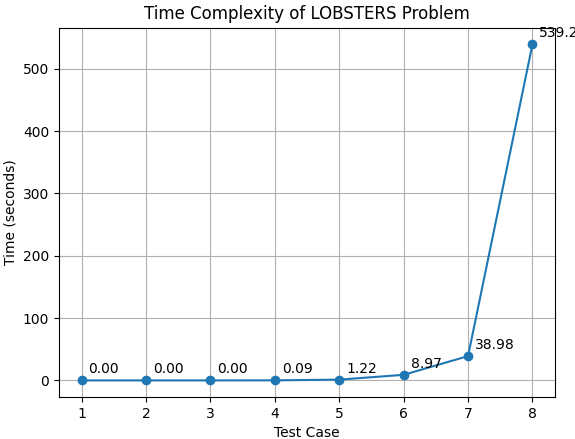
\includegraphics[width=\textwidth]{time_complexity_py.png}%
\end{figure}

%
\newpage%

       \vspace*{\fill}
                              
            From the complexity chart, we observe that Python is extremely fast on small ranges of data (data up to 10,000,000) for the first 7 cases, which is basically what we have expected to be.
         \vspace{2cm}
                           
            However, where are the tests 9 and 10 from the chart?
                        
\vspace{0.2cm}
            The answer is that the system is out of resources for such big computations for numbers bigger than 1,000,000,000.
            The numpy arrays cannot be computed for int64 data type, and even for the basic data types for 32-bit, we are having overflow.
\vspace{0.2cm}
            The encountered error when running the python script is (I will present the situation for test 9):
                        
            \begin{verbatim}
            numpy.core._exceptions._ArrayMemoryError: Unable to allocate 134. GiB for an array with shape 
            (6, 3000000001) and data type int64 ...
            \end{verbatim}

            So, running the actual dynamic programming algorithm for 10**9 entries with high capacities is not feasible on most machines 
            due to the massive memory and computational requirements. Instead, we typically use problem-specific optimizations or approximate methods for such large-scale problems.

            When we encounter an ArrayMemoryError from NumPy, the "134 GiB" refers to the amount of RAM (Random Access Memory) that the operation is attempting to allocate. 
            
            This is the primary memory that your computer uses to store data that is actively being worked on by the CPU.
\vspace{2cm}
            
            
            Further Explanation:

                        
\vspace{0.3cm}


            - Memory Allocation: When NumPy tries to create an array, it needs to allocate a continuous block of memory in RAM. 
                        
            - If the array is very large, the required memory might exceed the available RAM, causing the ArrayMemoryError.
\vspace{2cm}
            
                        
                        
            Why the Error Occurs:

                        
\vspace{0.3cm}

                        
            - Shape and Size: Your array has a shape of (6, 3,000,000,001) and each element is of type int64, which takes 8 bytes.  
                         
            - Memory calculation: Memory Required = 6 x 3,000,000,001 x 8 bytes ~ 144 GiB
\vspace{2cm}
            
                        
                        
           Proposed Solutions:

                        

\vspace{0.3cm}


            Of course, we have a lot of solutions for solving the memory problem and print the desired results.
            However, I propose 2 solutions:
\vspace{0.3cm}
                        

            1. Use the amount of free space from the SSD where you have installed your OS and use it for RAM memory allocation.
            It is not a fast solution and of course needs a big SSD, but it could make some wonders.
\vspace{0.2cm}
                        



            2. Use another algorithm for solving the lobsters problem, not dynamic programming or even greedy.
            A concatenation algorithm would fit into our situation, for example, something that works with digits of a number.
            For example, to obtain someway, somehow, every digit of the maximum value and print it digit by digit, like a string.
            Python has some modules that are working on this type of approach.
            
            
                        \vspace*{\fill}
        %
\newpage%


    \vspace*{\fill}

    
    \subsection{Is it C faster than Python ?}

                                   
    \vspace{1cm}
                        
    The answer is absolutely yes, speaking in general terms. And also on my dynamic programming implementation it is. 
                        

    BUT, the chart is made for the first 9 tests, despite where Python made only on the first 8 tests.
                        
                    
    What I want to say is that when 10**8 is exceeded it, on the test no.9 for example, it is not working.
                        

    It is not allocating memory for reading all the data from the csv for test no. 9 and moreover, of course, the output it is not as have we expected for no. 9.
    
                        
    It can be clearly seen in the chart that test no.9 is only almost 1.7 seconds on CPU time, meanwhile test no. 8 is 4.16 seconds on CPU.
    
                        
    This is showing us that something it is not working fine, because it can't take a shorter time for bigger data inputs to be computed.
\vspace{0.2cm}
    \vspace*{\fill}

   %


\begin{figure}[h!]%
\centering%
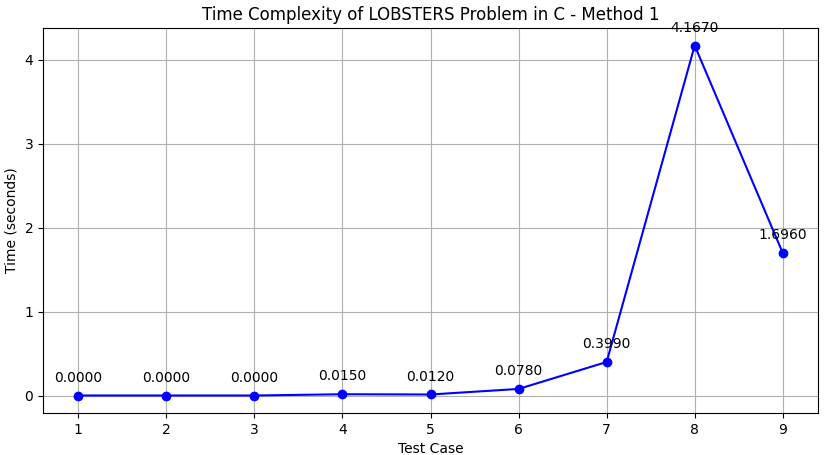
\includegraphics[width=\textwidth]{time_complexity_c_1.png}%
\end{figure}

%
\newpage%

    
    \vspace*{\fill}

    \subsection{Is C stable for all of the 10 testcases?}
                        
    \vspace{1cm}
    
    I would say NO. If we iterate and make computations for all 10 testcases, as we see in the chart and later from the output data, 
    the maximum values for each testcases are not correct... Firstly, from the chart, you see that the CPU times are making a "mountain peak",
    which is not what we expect from the chart... It was supposed to be continuely increasing.
   \vspace{0.2cm}
    \vspace*{\fill}    

    %


\begin{figure}[h!]%
\centering%
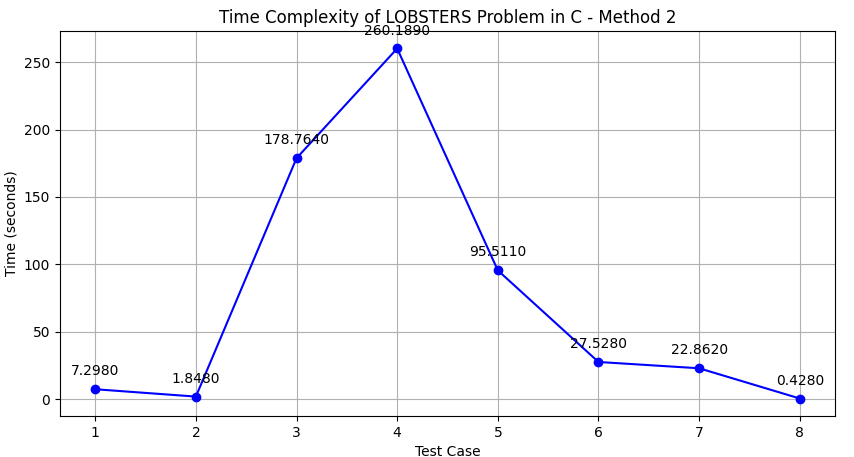
\includegraphics[width=\textwidth]{time_complexity_c_2.png}%
\end{figure}

%
\newpage%


    
    \vspace*{\fill}
                        
Computed output for subsection 4.2 : 
                        
\small
\begin{verbatim}
Test 1:
Max Value: 18
Selected Sizes: [8, 2, 1]
Selected Values: [9, 6, 3]
Time Elapsed: 0.0 seconds
                        
Test 2:
Max Value: 202
Selected Sizes: [86, 41, 36, 35]
Selected Values: [85, 69, 45, 3]
Time Elapsed: 0.0 seconds
                        
Test 3:
Max Value: 1846
Selected Sizes: [406, 390]
Selected Values: [957, 889]
Time Elapsed: 0.0 seconds
                        
Test 4:
Max Value: 27346
Selected Sizes: [3656, 2008, 1294]
Selected Values: [9950, 9424, 7972]
Time Elapsed: 0.09375 seconds
                        
Test 5:
Max Value: 267015
Selected Sizes: [89010, 55362, 22895, 19402, 5095]
Selected Values: [82640, 65938, 57042, 42824, 18571]
Time Elapsed: 1.21875 seconds
                        
Test 6:
Max Value: 2459703
Selected Sizes: [867711, 559535, 540254]
Selected Values: [973447, 882122, 604134]
Time Elapsed: 8.96875 seconds
                        
Test 7:
Max Value: 14148044
Selected Sizes: [6751549, 2220561]
Selected Values: [9435450, 4712594]
Time Elapsed: 38.984375 seconds
                        
Test 8:
Max Value: 139189354
Selected Sizes: [35495527, 17034213, 2956034]
Selected Values: [78534293, 53816377, 6838684]
Time Elapsed: 539.203125 seconds
                        
\end{verbatim}


As I was talking in subsection 4.2 , it makes the chart only for the first 8 testcases because the cpu times are continuely increasing,
and that's because I set into the "experimental data" folder, "results" python file to take into computation only 8 cases, not all 10. 

Otherwise,it was raising the overflow error that I was saying. 
                        

**(I used results.py and results.c for this testing because not to destroy my application, these files are only for this report)**
                        
    \vspace*{\fill}

    
%
\newpage%


   \vspace*{\fill}
                        
Computed output for subsection 4.3 :
                        
\small
\begin{verbatim}
Test 1:
Max Value: 18
Selected Sizes: 8 1 2 
Selected Values: 3 6 9 
Time Elapsed: 0.000000 seconds
                        
Test 2:
Max Value: 202
Selected Sizes: 41 86 35 36 
Selected Values: 69 45 85 3 
Time Elapsed: 0.000000 seconds
                        
Test 3:
Max Value: 1846
Selected Sizes: 406 390 
Selected Values: 957 889 
Time Elapsed: 0.000000 seconds
                        
Test 4:
Max Value: 27346
Selected Sizes: 3656 2008 1294 
Selected Values: 7972 9424 9950 
Time Elapsed: 0.015000 seconds
                        
Test 5:
Max Value: 267015
Selected Sizes: 19402 5095 55362 22895 89010 
Selected Values: 57042 42824 65938 18571 82640 
Time Elapsed: 0.012000 seconds
                        
Test 6:
Max Value: 2459703
Selected Sizes: 867711 559535 540254 
Selected Values: 882122 604134 973447 
Time Elapsed: 0.078000 seconds
                        
Test 7:
Max Value: 14148044
Selected Sizes: 6751549 2220561 
Selected Values: 9435450 4712594 
Time Elapsed: 0.399000 seconds
                        
Test 8:
Max Value: 139189354
Selected Sizes: 17034213 2956034 35495527 
Selected Values: 53816377 78534293 6838684 
Time Elapsed: 4.167000 seconds
                        
Test 9:
Max Value: 102015200
Selected Sizes: 10000000 200000 900 14 
Selected Values: 100000000 2000000 15000 200 
Time Elapsed: 1.696000 seconds
                        
\end{verbatim}
                        

For subsection 4.3 it is printing the expected outputs, less than testcase no. 9, 
where it is not reading the selected sizes and values correctly, 
beacuse they are exceeding 100.000.000 (10**8).
                        
                        
   \vspace*{\fill}

%
\newpage%

 \vspace*{\fill}
Computed output for subsection 4.4 : 
                         
\small
\begin{verbatim}                     
Test 1:
Max Value: 20
Selected Sizes: 8 7 1 2 
Selected Values: 3 2 6 9 
Time Elapsed: 7.298000 seconds
                        
Test 2:
Max Value: 231
Selected Sizes: 41 86 35 36 48 
Selected Values: 69 45 85 3 29 
Time Elapsed: 1.848000 seconds
                        
Test 3:
Max Value: 2462
Selected Sizes: 406 603 594 390 505 
Selected Values: 957 178 338 889 100 
Time Elapsed: 178.764000 seconds
                        
Test 4:
Max Value: 37411
Selected Sizes: 8549 3656 2008 9642 1294 
Selected Values: 6050 7972 9424 4015 9950 
Time Elapsed: 260.189000 seconds
                        
Test 5:
Max Value: 267015
Selected Sizes: 19402 5095 55362 22895 89010 
Selected Values: 57042 42824 65938 18571 82640 
Time Elapsed: 95.511000 seconds
                        
Test 6:
Max Value: 3658526
Selected Sizes: 867711 980461 929169 559535 540254 
Selected Values: 882122 271492 927331 604134 973447 
Time Elapsed: 27.528000 seconds

Test 7:
Max Value: 32427822
Selected Sizes: 6751549 6116514 9756838 2220561 4155287 
Selected Values: 9435450 6511279 6183077 4712594 5585422 
Time Elapsed: 22.862000 seconds

Test 8:
Max Value: 78534293
Selected Sizes: 2956034 
Selected Values: 78534293 
Time Elapsed: 0.428000 seconds
                        
\end{verbatim}


So, as I said on the 4.4 subsection chart this is the result for each testcase, and everything here is wrong.
                        
Why the output it is not as expected?


Because C is basically trying to compute all the tescases, so it speeds up the process and every testcase is printing some of the variants
for the max value, but not the correct one.                

Python tells us that we are out of memory and computes everything as clean as possible, but C is trying to compute everything even if it is not correct.

That's why Python is better... And that's the subjective part from my point of view. 

It is telling us exactly what we are doing, not trying to "impress" us.                   

 \vspace*{\fill}
%
\newpage%

\vspace*{\fill}
                        
\subsection{Conducted results on Test no. 11}

                        \vspace{1 cm}           
This section it is written only for the purpose on how it is working the algorithm.
                        
It searches the sizes with max values that their sum not exceed the fishing-net capacity.
                        
When the best combination is reached, we print the max value, the sum of sizes, and the sum of values.
                        
\small
\begin{verbatim}                     
    
No. of tests: 3
No. of lobsters: 10
Maximum value for random data: 100
Net capacity: 129


Lobsters data:
Test no. 1: [29, 77] [42, 25] [33, 39] [17, 10] [83, 43] [18, 1] [35, 54] [81, 77] [89, 34] [22, 88] 
Test no. 2: [59, 68] [61, 36] [58, 79] [10, 19] [47, 59] [20, 81] [3, 75] [89, 60] [24, 89] [4, 59] 
Test no. 3: [8, 68] [18, 59] [97, 42] [42, 35] [91, 59] [47, 60] [25, 4] [49, 22] [47, 74] [0, 75] 


Sizes:
Test no. 1 : 29 42 33 17 83 18 35 81 89 22 
Test no. 2 : 59 61 58 10 47 20 3 89 24 4 
Test no. 3 : 8 18 97 42 91 47 25 49 47 0 

Values:
Test no. 1 : 77 25 39 10 43 1 54 77 34 88 
Test no. 2 : 68 36 79 19 59 81 75 60 89 59 
Test no. 3 : 68 59 42 35 59 60 4 22 74 75 

Maximum value of capture per test:

Test no. 1:
Maximum value: 258
Sizes: 35 + 33 + 29 + 22 = 119
Values: 88 + 77 + 54 + 39 = 258

Test no. 2:
Maximum value: 402
Sizes: 58 + 24 + 20 + 10 + 4 + 3 = 119
Values: 89 + 81 + 79 + 75 + 59 + 19 = 402

Test no. 3:
Maximum value: 336
Sizes: 47 + 47 + 18 + 8 = 120
Values: 75 + 74 + 68 + 60 + 59 = 336
    
                        
    \end{verbatim}                    
\vspace*{\fill}
%
\newpage%

        \vspace*{\fill}
        \begin{center}
            \LARGE \textbf{Thank you for your time!} \\
            \LARGE \textbf{- TECHNICAL REPORT ENDED -}
        \end{center}
                 
        \vspace*{\fill}
    %
Github repository link %
\href{https://github.com/necsulea-andrei-ace-ucv/TEMA_DE_CASA_AD}{click here}%
\end{document}